\section{Question 4-6: Dimensionality Reduction}

\subsection{Features Relationship}

The \emph{correlation matrix} is a matrix represent the correlation coeficient of different features.
The matrix shows the correlation between all pairs of features within the dataset.
We use the correlation matrix to summarise the relationship of the given dataset and to visualise patterns within (see Figure \ref{Fig: Correlation Heatmap}).


\begin{figure}
    \centering
    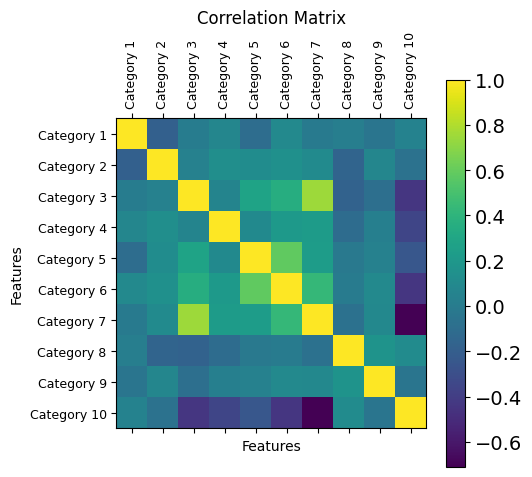
\includegraphics[width=0.75\textwidth]{Appendices/corr.png}
    \caption{Correlation of each features visualised as a heatmap}
    \label{Fig: Correlation Heatmap}
\end{figure}

\subsection{Dimensional Reduction and Data Loss}

The given data of 10 features can be describe by 2 vectors using the Principal Component analysis procedure.
The relation between the two vectors can be described in a 2D plot with a linear regression line to describe the trend of the two principal components (see Figure \ref{Fig: PCA}).

Dimensional reduction would also introduce information loss.
In the given dataset, we have reconstructed the data from 2 dimensions to 10 dimension, results shows that there are 75\% of data are mismatched with the original data.

\begin{figure}
    \centering
    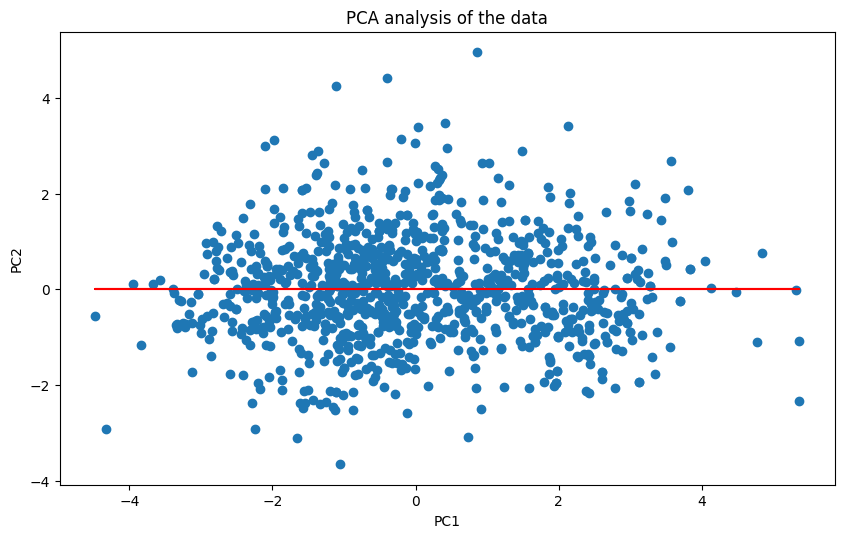
\includegraphics[width=\textwidth]{Appendices/PCA-Reg.png}
    \caption{Principal Components analysis reduces 10 dimentsions to 2 dimentsions, the regression line describe the trend of those components}
    \label{Fig: PCA}
\end{figure}

\begin{lstlisting}[language=Python]
# Perform data reconstruction
Xrex = pca.inverse_transform(Zred)
print(f'Reconstructed data shape: {Xrex.shape}')

# Measure the reconstruction error
rec_error = np.linalg.norm(Xnorm - Xrex) / np.linalg.norm(Xnorm)
print(f'Reconstruction error: {rec_error}')

>>>Reconstructed data shape: (980, 10)
>>>Reconstruction error: 0.7589269810329784
\end{lstlisting}

\subsection{Explained Variance Percentage}

\textbf{Explained variance} is a measurement for how much variance can be attributed from the dataset to each of the principal components (also known as eigenvectors) \cite{o1982measures}.
For example, a dataset with 10 dimension can be explained by two component, the first component can explain 20% of the variance, and the other component explain the rest of 80%.

We can calculate the explained variance by a function of ratio.
For a $n$ eigenvectors, the related eigenvalue $\lambda_i$ and the sum of all eigenvalues, we calculate the explained variance with the following formula:

\begin{equation}
    \frac{\lambda_i}{\sum^n_{j=1}\lambda_j}
\end{equation}

